
%%%%%%%%%%%%%%%%%%%%%%%%%%%%%%%%%%%%%%%%%%%%%%%%%%%%%%%%%%%%%%%%%%%%%%%%%%%%%%%%%%
\begin{frame}[fragile]\frametitle{}

\begin{center}
{\Large Text Processing Pipeline with Nltk}
\end{center}
\end{frame}

%%%%%%%%%%%%%%%%%%%%%%%%%%%%%%%%%%%%%%%%%%%%%%%%%%%%%%%%%%%%%%%%%%%%%%%%%%%%%%%%%%
\begin{frame}[fragile]\frametitle{NLP Pipeline}

\begin{itemize}
\item Tokenization
\item Stemming
\item Lemmatization
\item Tagging
\item Parsing 
\item Chunking 
\item Adding missing fields 
\end{itemize}
\end{frame}

%%%%%%%%%%%%%%%%%%%%%%%%%%%%%%%%%%%%%%%%%%%%%%%%%%%%%%%%%%%%%%%%%%%%%%%%%%%%%%%%%%
\begin{frame}[fragile]
\frametitle{Tokenization}
\begin{itemize}
\item Whitespace often do not indicate a word break: sometime we may want to lump together words that are separated by a white space  (whitespace?) but that we want to regard as a single word
\item San Francisco
\item The New York-New Heaven railroad
\item Wake up, work out
\end{itemize}
\end{frame}

%%%%%%%%%%%%%%%%%%%%%%%%%%%%%%%%%%%%%%%%%%%%%%%%%%%%%%%%%%%%%%%%%%%%%%%%%%%%%%%%%%
\begin{frame}[fragile]
\frametitle{Tokenization}
\begin{center}
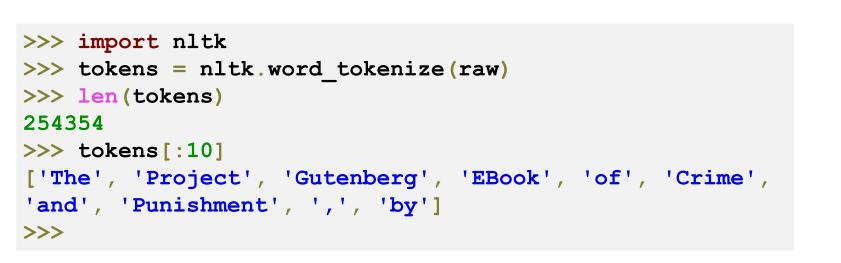
\includegraphics[width=\linewidth,keepaspectratio]{dataweb2}
\end{center}
What is the $type()$ of the tokens?
\end{frame}

%%%%%%%%%%%%%%%%%%%%%%%%%%%%%%%%%%%%%%%%%%%%%%%%%%%%%%%%%%%%%%%%%%%%%%%%%%%%%%%%%%
\begin{frame}[fragile]
\frametitle{ Regular Expressions for Detecting Word Patterns }
\begin{itemize}
\item Many linguistic processing tasks involve pattern matching. 
\item Regular expressions (RE) give us a powerful and flexible method for describing the character patterns we are interested in.
\item To use regular expressions in Python we need to import the $re$ library using: \lstinline|import re|

\begin{center}
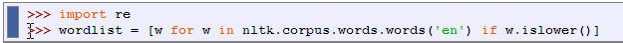
\includegraphics[width=\linewidth,keepaspectratio]{re1}
\end{center}
\item $re.search(p,s)$ is a function to check whether the pattern p can be found somewhere inside the string $s$. 
\begin{center}
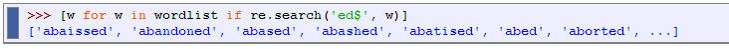
\includegraphics[width=\linewidth,keepaspectratio]{re2}
\end{center}
\end{itemize}
\end{frame}

%%%%%%%%%%%%%%%%%%%%%%%%%%%%%%%%%%%%%%%%%%%%%%%%%%%%%%%%%%%%%%%%%%%%%%%%%%%%%%%%%%%
%\begin{frame}\frametitle{Regular Expressions}
%\begin{itemize}
%\item string matching
%\item substitution
%\item patterns, classes
%\item Python's regular expression module: \texttt{re}
%\item NLTK's utility function: \texttt{re\_show}
%\end{itemize}
%\end{frame}


%%%%%%%%%%%%%%%%%%%%%%%%%%%%%%%%%%%%%%%%%%%%%%%%%%%%%%%%%%%%%%%%%%%%%%%%%%%%%%%%%%
\begin{frame}[fragile]
\frametitle{Regular Expressions}
Basic Regular Expression Meta-Characters 
\begin{center}
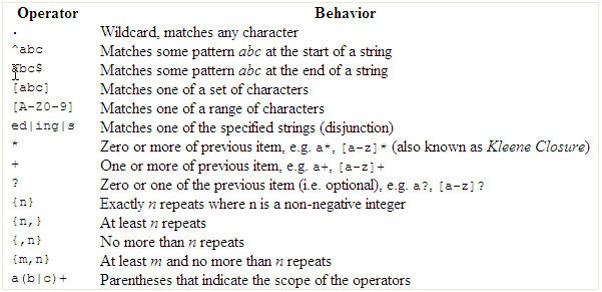
\includegraphics[width=\linewidth,keepaspectratio]{re3}
\end{center}
\end{frame}


%%%%%%%%%%%%%%%%%%%%%%%%%%%%%%%%%%%%%%%%%%%%%%%%%%%%%%%%%%%%%%%%%%%%%%%%%%%%%%%%%%
\begin{frame}[fragile]\frametitle{Loading module, Matching}
\begin{itemize}
\item Set up:

{\small
\begin{lstlisting}
  >>> import nltk, re
  >>> sent = ''colourless green ideas sleep furiously''
\end{lstlisting}}

\item Matching:

{\small
\begin{lstlisting}
  >>> nltk.re_show('l', sent)
  co{l}our{l}ess green ideas s{l}eep furious{l}y
  >>> nltk.re_show(`green', sent)
  colourless {green} ideas sleep furiously
\end{lstlisting}}
\end{itemize}
\end{frame}

%%%%%%%%%%%%%%%%%%%%%%%%%%%%%%%%%%%%%%%%%%%%%%%%%%%%%%%%%%%%%%%%%%%%%%%%%%%%%%%%%%
\begin{frame}[fragile]\frametitle{Substitutions}

\begin{itemize}
\item E.g. replace all instances of \texttt{l} with \texttt{s}.
\item Creates an output string (doesn't modify input)

\begin{lstlisting}
  >>> re.sub('l', 's', sent)
  'cosoursess green ideas sseep furioussy'
\end{lstlisting}

\item Work on substrings (NB not words)

\begin{lstlisting}
  >>> re.sub('green', 'red', sent)
  'colourless red ideas sleep furiously'
\end{lstlisting}
\end{itemize}
\end{frame}

%%%%%%%%%%%%%%%%%%%%%%%%%%%%%%%%%%%%%%%%%%%%%%%%%%%%%%%%%%%%%%%%%%%%%%%%%%%%%%%%%%
\begin{frame}[fragile]\frametitle{More Complex Patterns}

\begin{itemize}
\item Disjunction:

{\small
\begin{lstlisting}
  >>> nltk.re_show('(green|sleep)', sent)
  colourless {green} ideas {sleep} furiously
  >>> re.findall('(green|sleep)', sent)
  ['green', 'sleep']
\end{lstlisting}}

\item Character classes, e.g. non-vowels followed by vowels:

{\small
\begin{lstlisting}
  >>> nltk.re_show('[^aeiou][aeiou]', sent)
  {co}{lo}ur{le}ss g{re}en{ i}{de}as s{le}ep {fu}{ri}ously
  >>> re.findall('[^aeiou][aeiou]', sent)
  ['co', 'lo', 'le', 're', ' i', 'de', 'le', 'fu', 'ri']
\end{lstlisting}}
\end{itemize}
\end{frame}

%%%%%%%%%%%%%%%%%%%%%%%%%%%%%%%%%%%%%%%%%%%%%%%%%%%%%%%%%%%%%%%%%%%%%%%%%%%%%%%%%%
\begin{frame}[fragile]\frametitle{Structured Results}
\begin{itemize}
\item Select a sub-part to be returned
\item e.g. non-vowel characters which appear before a vowel:

{\small
\begin{lstlisting}
  >>> re.findall('([^aeiou])[aeiou]', sent)
  ['c', 'l', 'l', 'r', ' ', 'd', 'l', 'f', 'r']
\end{lstlisting}}

\item generate \textit{tuples}, for later tabulation

{\small
\begin{lstlisting}
  >>> re.findall('([^aeiou])([aeiou])', sent)
  [('c', 'o'), ('l', 'o'), ('l', 'e'), ('r', 'e'), (' ', 'i'), ('d', 'e'), ('l', 'e'), ('f', 'u'), ('r', 'i')]
\end{lstlisting}}
\end{itemize}
\end{frame}

%%%%%%%%%%%%%%%%%%%%%%%%%%%%%%%%%%%%%%%%%%%%%%%%%%%%%%%%%%%%%%%%%%%%%%%%%%%%%%%%%%
\begin{frame}[fragile]
\frametitle{RE for Tokenizing Text: By space}
\begin{center}
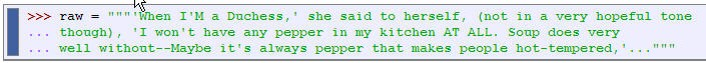
\includegraphics[width=\linewidth,keepaspectratio]{re10}

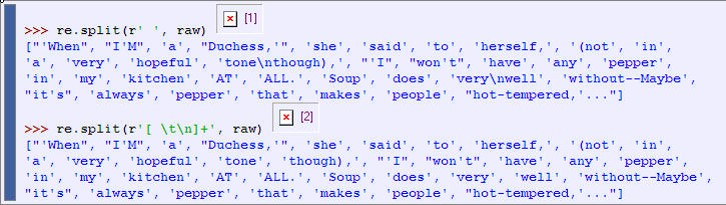
\includegraphics[width=\linewidth,keepaspectratio]{re11}

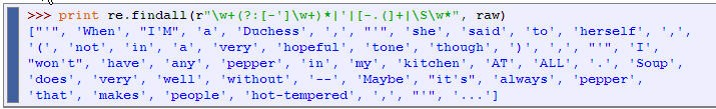
\includegraphics[width=\linewidth,keepaspectratio]{re12}
\end{center}
\end{frame}

%%%%%%%%%%%%%%%%%%%%%%%%%%%%%%%%%%%%%%%%%%%%%%%%%%%%%%%%%%%%%%%%%%%%%%%%%%%%%%%%%%
\begin{frame}[fragile]
\frametitle{NLTK's Regular Expression Tokenizer }
\begin{center}
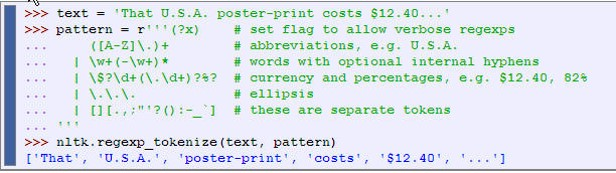
\includegraphics[width=\linewidth,keepaspectratio]{re13}
\end{center}
\end{frame}


%%%%%%%%%%%%%%%%%%%%%%%%%%%%%%%%%%%%%%%%%%%%%%%%%%%%%%%%%%%%%%%%%%%%%%%%%%%%%%%%%%
\begin{frame}[fragile]
\frametitle{ Sentence Segmentation with nltk }
\begin{itemize}
\item Some corpora already provide access at the sentence level. 
\item In the following example, we compute the average number of words per sentence in the Brown Corpus:
\begin{center}
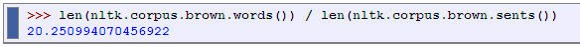
\includegraphics[width=\linewidth,keepaspectratio]{sent1}
\end{center}
\end{itemize}
\end{frame}

%%%%%%%%%%%%%%%%%%%%%%%%%%%%%%%%%%%%%%%%%%%%%%%%%%%%%%%%%%%%%%%%%%%%%%%%%%%%%%%%%%
\begin{frame}[fragile]
\frametitle{Normalization: Stopwords}
\begin{lstlisting}
from nltk.corpus import stopwords
    stopwords = nltk.corpus.stopwords.words('english')
    content = [w.lower() for w in text 
               if w.lower() not in stopwords \ # w should not be in NLTK stopwords
                   and w.isalpha() \ # w should consists of letters, not numbers, not punctuation
                   and w.lower() not in hapaxes] # w should have frequency > 1 
\end{lstlisting}
\end{frame}

%%%%%%%%%%%%%%%%%%%%%%%%%%%%%%%%%%%%%%%%%%%%%%%%%%%%%%%%%%%%%%%%%%%%%%%%%%%%%%%%%%
\begin{frame}[fragile]
\frametitle{Punkt sentence segmenter }
\begin{center}
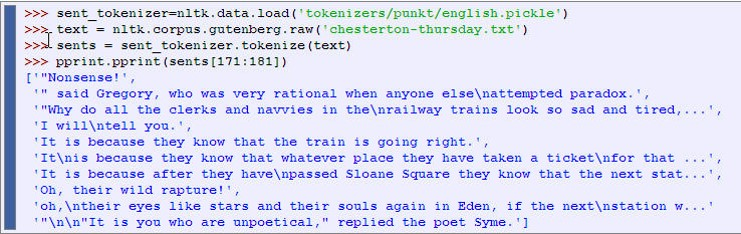
\includegraphics[width=\linewidth,keepaspectratio]{sent2}
\end{center}
\end{frame}



%%%%%%%%%%%%%%%%%%%%%%%%%%%%%%%%%%%%%%%%%%%%%%%%%%%%%%%%%%%%%%%%%%%%%%%%%%%%%%%%%%
\begin{frame}[fragile]
\frametitle{ Regular Expressions for Stemming }
\begin{center}
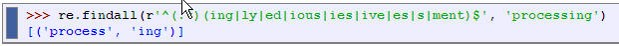
\includegraphics[width=\linewidth,keepaspectratio]{re4}

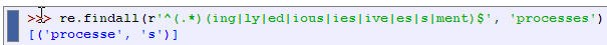
\includegraphics[width=\linewidth,keepaspectratio]{re5}
\end{center}
Note: the star operator is ''greedy'' and the .* part of the expression tries to consume as much of the input as possible. If we use the ''non-greedy'' version of the star operator, written *?, we get what we want: 
\begin{center}
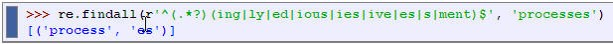
\includegraphics[width=\linewidth,keepaspectratio]{re6}
\end{center}
\end{frame}

%%%%%%%%%%%%%%%%%%%%%%%%%%%%%%%%%%%%%%%%%%%%%%%%%%%%%%%%%%%%%%%%%%%%%%%%%%%%%%%%%%
\begin{frame}[fragile]
\frametitle{ Regular Expressions for Stemming }
Let's define a function to perform stemming, and apply it to a whole text

\begin{center}
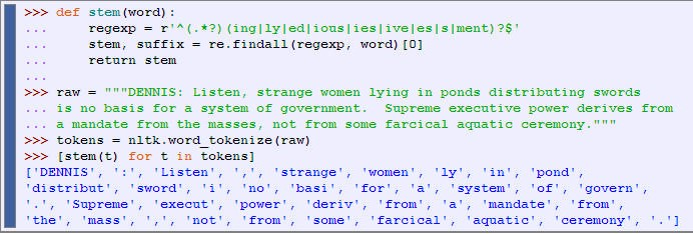
\includegraphics[width=\linewidth,keepaspectratio]{re7}
\end{center}
The RE removed the s from ponds but also from is and basis. It produced some non-words like distribut and deriv, but these are acceptable stems in some applications.
\end{frame}

%%%%%%%%%%%%%%%%%%%%%%%%%%%%%%%%%%%%%%%%%%%%%%%%%%%%%%%%%%%%%%%%%%%%%%%%%%%%%%%%%%
\begin{frame}[fragile]
\frametitle{ NLTK Stemmers }
\begin{itemize}
\item NLTK includes several off-the-shelf stemmers. The Porter and Lancaster stemmers follow their own rules for stripping affixes. 
\item Stemming is not a well-defined process, and we typically pick the stemmer that best suits the application we have in mind. 
\end{itemize}
\begin{center}
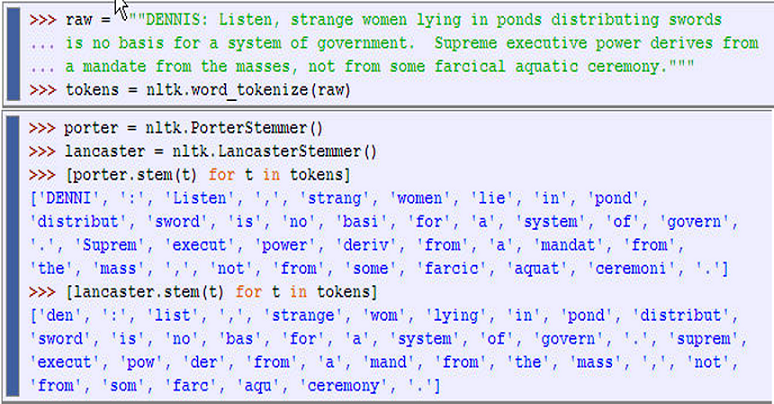
\includegraphics[width=0.8\linewidth,keepaspectratio]{nltkstem1}
\end{center}
\end{frame}

%%%%%%%%%%%%%%%%%%%%%%%%%%%%%%%%%%%%%%%%%%%%%%%%%%%%%%%%%%%%%%%%%%%%%%%%%%%%%%%%%%
\begin{frame}[fragile]
\frametitle{ NLTK Lemmatization }
\begin{lstlisting}
raw = """DENNIS: Listen, strange women lying in ponds distributing swords
is no basis for a system of government.  Supreme executive power derives from
a mandate from the masses, not from some farcical aquatic ceremony."""
tok = nltk.word_tokenize(raw)

wnl = nltk.WordNetLemmatizer()
lemmatized =  [wnl.lemmatize(t) for t in tok]
print " ".join(lemmatized) 
\end{lstlisting}
\end{frame}

%%%%%%%%%%%%%%%%%%%%%%%%%%%%%%%%%%%%%%%%%%%%%%%%%%%%%%%%%%%%%%%%%%%%%%%%%%%%%%%%%%
\begin{frame}[fragile]
\frametitle{ WordNet Try outs}
\begin{lstlisting}
from nltk.corpus import wordnet as wn

print wn.synsets('dog')
>>>[Synset('dog.n.01'), Synset('frump.n.01'), Synset('dog.n.03'), Synset('cad.n.01'), Synset('frank.n.02'), Synset('pawl.n.01'), Synset('andiron.n.01'), Synset('chase.v.01')]

wn.synsets('dog', pos=wn.VERB)
>>>[Synset('chase.v.01')]

wn.synset('dog.n.01')
>>>Synset('dog.n.01')
\end{lstlisting}
\end{frame}

%%%%%%%%%%%%%%%%%%%%%%%%%%%%%%%%%%%%%%%%%%%%%%%%%%%%%%%%%%%%%%%%%%%%%%%%%%%%%%%%%%
\begin{frame}[fragile]
\frametitle{ WordNet Try outs}
\begin{lstlisting}
print(wn.synset('dog.n.01').definition)
a member of the genus Canis (probably descended from the common wolf) that has been domesticated by man since prehistoric times; occurs in many breeds

print(wn.synset('dog.n.01').examples[0])
>>>the dog barked all night

print wn.synset('dog.n.01').lemmas
>>>[Lemma('dog.n.01.dog'), Lemma('dog.n.01.domestic_dog'), Lemma('dog.n.01.Canis_familiaris')]
\end{lstlisting}
\end{frame}

%%%%%%%%%%%%%%%%%%%%%%%%%%%%%%%%%%%%%%%%%%%%%%%%%%%%%%%%%%%%%%%%%%%%%%%%%%%%%%%%%%
\begin{frame}[fragile]
\frametitle{ WordNet Try outs}
\begin{lstlisting}
#if we know a lemma, then we can get the corresponding synset
wn.lemma('dog.n.01.dog').synset
>>>Synset('dog.n.01')

#Synsets are words that share a common meaning. There are various relations within Synsets for e.g. 
dog = wn.synset('dog.n.01')
print dog.hypernyms()
>>>[Synset('domestic_animal.n.01'), Synset('canine.n.02')]
\end{lstlisting}
\end{frame}

%%%%%%%%%%%%%%%%%%%%%%%%%%%%%%%%%%%%%%%%%%%%%%%%%%%%%%%%%%%%%%%%%%%%%%%%%%%%%%%%%%
\begin{frame}[fragile]
\frametitle{ WordNet Semantic similarity}
Given a particular synset, we can traverse the WordNet network to find synsets with related meanings.
\begin{lstlisting}
right = wn.synset('right_whale.n.01')
orca = wn.synset('orca.n.01')
minke = wn.synset('minke_whale.n.01')
tortoise = wn.synset('tortoise.n.01')
novel = wn.synset('novel.n.01')

right.lowest_common_hypernyms(minke)
>>>[Synset('baleen_whale.n.01')]

right.lowest_common_hypernyms(orca)
>>>[Synset('whale.n.02')]

right.lowest_common_hypernyms(tortoise)
>>>[Synset('vertebrate.n.01')]
\end{lstlisting}
\end{frame}

%%%%%%%%%%%%%%%%%%%%%%%%%%%%%%%%%%%%%%%%%%%%%%%%%%%%%%%%%%%%%%%%%%%%%%%%%%%%%%%%%%
\begin{frame}[fragile]\frametitle{}

\begin{center}
{\Large Text Processing Example}
\end{center}

{\tiny (Ref: How to Clean Text for Machine Learning with Python - Jason Brownlee and Text Preprocessing in Python: Steps, Tools, and Examples - Data Monsters)}
\end{frame}

%%%%%%%%%%%%%%%%%%%%%%%%%%%%%%%%%%%%%%%%%%%%%%%%%%%%%%%%%%%%%%%%%%%%%%%%%%%%%%%%%%
\begin{frame}[fragile]\frametitle{Dataset}
Metamorphosis by Franz Kafka
\begin{itemize}
\item Book ``Metamorphosis'' by Franz Kafka
\item The full text for Metamorphosis is available for free from Project Gutenberg. http://www.gutenberg.org/ebooks/5200
\item You can download the ASCII text version of the text here: http://www.gutenberg.org/cache/epub/5200/pg5200.txt
\item Download the file and place it in your current working directory with the file name ``metamorphosis.txt''.
\end{itemize}
\end{frame}

%%%%%%%%%%%%%%%%%%%%%%%%%%%%%%%%%%%%%%%%%%%%%%%%%%%%%%%%%%%%%%%%%%%%%%%%%%%%%%%%%%
\begin{frame}[fragile]\frametitle{Manual Cleaning}
\begin{itemize}
\item The file contains header and footer information that we are not interested in, specifically copyright and license information. Open the file and delete the header and footer information and save the file as ``metamorphosis\_clean.txt''.

\item The start of the clean file should look like:

``One morning, when Gregor Samsa woke from troubled dreams, he found himself transformed in his bed into a horrible vermin.''

\item The file should end with:

``And, as if in confirmation of their new dreams and good intentions, as soon as they reached their destination Grete was the first to get up and stretch out her young body.''
\end{itemize}
\end{frame}


%%%%%%%%%%%%%%%%%%%%%%%%%%%%%%%%%%%%%%%%%%%%%%%%%%%%%%%%%%%%%%%%%%%%%%%%%%%%%%%%%%
\begin{frame}[fragile]\frametitle{Some Observations}
\begin{itemize}
\item It’s plain text so there is no markup to parse (yay!).
\item The translation of the original German uses UK English (e.g. “travelling“).
\item The lines are artificially wrapped with new lines at about 70 characters (meh).
\item There are no obvious typos or spelling mistakes.
\item There’s punctuation like commas, apostrophes, quotes, question marks, and more.
\item There’s hyphenated descriptions like “armour-like”.
\item There’s a lot of use of the em dash (“-“) to continue sentences (maybe replace with commas?).
\item There are names (e.g. “Mr. Samsa“)
\item There does not appear to be numbers that require handling (e.g. 1999)
\item There are section markers (e.g. “II” and “III”), and we have removed the first “I”.
\end{itemize}
\end{frame}

%%%%%%%%%%%%%%%%%%%%%%%%%%%%%%%%%%%%%%%%%%%%%%%%%%%%%%%%%%%%%%%%%%%%%%%%%%%%%%%%%%
\begin{frame}[fragile]
\frametitle{Load Data}
\begin{lstlisting}
# load data
filename = 'metamorphosis_clean.txt'
file = open(filename, 'rt')
text = file.read()
file.close()
\end{lstlisting}
``text'' will be used for further processing.
\end{frame}


%%%%%%%%%%%%%%%%%%%%%%%%%%%%%%%%%%%%%%%%%%%%%%%%%%%%%%%%%%%%%%%%%%%%%%%%%%%%%%%%%%
\begin{frame}[fragile]
\frametitle{ Split into Sentences}
A good useful first step is to split the text into sentences.
\begin{lstlisting}
# split into sentences
from nltk import sent_tokenize
sentences = sent_tokenize(text)
print(sentences[0])
\end{lstlisting}
\end{frame}


%%%%%%%%%%%%%%%%%%%%%%%%%%%%%%%%%%%%%%%%%%%%%%%%%%%%%%%%%%%%%%%%%%%%%%%%%%%%%%%%%%
\begin{frame}[fragile]
\frametitle{ Split into Words}
Splits tokens based on white space and punctuation. For example, commas and periods are taken as separate tokens. Contractions are split apart (e.g. “What’s” becomes “What” “‘s“). Quotes are kept, and so on.
\begin{lstlisting}
# split into words
from nltk.tokenize import word_tokenize
tokens = word_tokenize(text)
print(tokens[:100])
\end{lstlisting}
\end{frame}

%%%%%%%%%%%%%%%%%%%%%%%%%%%%%%%%%%%%%%%%%%%%%%%%%%%%%%%%%%%%%%%%%%%%%%%%%%%%%%%%%%
\begin{frame}[fragile]
\frametitle{ Filter Out Punctuation}
Filter out all tokens that we are not interested in, such as all standalone punctuation.
\begin{lstlisting}
# remove all tokens that are not alphabetic
words = [word for word in tokens if word.isalpha()]
print(words[:100])
\end{lstlisting}
\end{frame}


%%%%%%%%%%%%%%%%%%%%%%%%%%%%%%%%%%%%%%%%%%%%%%%%%%%%%%%%%%%%%%%%%%%%%%%%%%%%%%%%%%
\begin{frame}[fragile]
\frametitle{Filter out Stop Words}
Stop words are those words that do not contribute to the deeper meaning of the phrase.
They are the most common words such as: “the“, “a“, and “is“.
\begin{lstlisting}
from nltk.corpus import stopwords
stop_words = stopwords.words('english')
print(stop_words)

['i', 'me', 'my', 'myself', 'we', 'our', 'ours', 'ourselves', 'you', 'your', 'yours', 'yourself', 'yourselves', 'he', 'him', 'his', 'himself', 'she', 'her', 'hers', 'herself', 'it', 'its', 'itself', 'they', 'them', 'their', 'theirs', 'themselves', 'what', 'which', 'who', 'whom', 'this', 'that', 'these', 'those', 'am', 'is', 'are', 'was', 'were', 'be', 'been', 'being', 'have', 'has', 'had', 'having', 'do', 'does', 'did', 'doing', 'a', 'an', 'the', 'and', 'but', 'if', 'or', 'because', 'as', 'until', 'while', 'of', 'at', 'by', 'for', 'with', 'about', 'against', 'between', 'into', 'through', 'during', 'before', 'after', 'above', 'below', 'to', 'from', 'up', 'down', 'in', 'out', 'on', 'off', 'over', 'under', 'again', 'further', 'then', 'once', 'here', 'there', 'when', 'where', 'why', 'how', 'all', 'any', 'both', 'each', 'few', 'more', 'most', 'other', 'some', 'such', 'no', 'nor', 'not', 'only', 'own', 'same', 'so', 'than', 'too', 'very', 's', 't', 'can', 'will', 'just', 'don', 'should', 'now', 'd', 'll', 'm', 'o', 're', 've', 'y', 'ain', 'aren', 'couldn', 'didn', 'doesn', 'hadn', 'hasn', 'haven', 'isn', 'ma', 'mightn', 'mustn', 'needn', 'shan', 'shouldn', 'wasn', 'weren', 'won', 'wouldn']
\end{lstlisting}
Filter them
\begin{lstlisting}
words = [w for w in words if not w in stop_words]
print(words[:100])
\end{lstlisting}
\end{frame}

%%%%%%%%%%%%%%%%%%%%%%%%%%%%%%%%%%%%%%%%%%%%%%%%%%%%%%%%%%%%%%%%%%%%%%%%%%%%%%%%%%
\begin{frame}[fragile]
\frametitle{Stem Words}
Stemming refers to the process of reducing each word to its root or base.
For example “fishing,” “fished,” “fisher” all reduce to the stem “fish.”
\begin{lstlisting}
# stemming of words
from nltk.stem.porter import PorterStemmer
porter = PorterStemmer()
stemmed = [porter.stem(word) for word in tokens]
print(stemmed[:100])
\end{lstlisting}
There is a nice suite of stemming and lemmatization algorithms to choose from in NLTK, if reducing words to their root is something you need for your project.
\end{frame}


%%%%%%%%%%%%%%%%%%%%%%%%%%%%%%%%%%%%%%%%%%%%%%%%%%%%%%%%%%%%%%%%%%%%%%%%%%%%%%%%%%
\begin{frame}[fragile]
\frametitle{Stem Words}
Stemming refers to the process of reducing each word to its root or base.
For example “fishing,” “fished,” “fisher” all reduce to the stem “fish.”
\begin{lstlisting}
# stemming of words
from nltk.stem.porter import PorterStemmer
porter = PorterStemmer()
stemmed = [porter.stem(word) for word in tokens]
print(stemmed[:100])
\end{lstlisting}
There is a nice suite of stemming and lemmatization algorithms to choose from in NLTK, if reducing words to their root is something you need for your project.
\end{frame}


%%%%%%%%%%%%%%%%%%%%%%%%%%%%%%%%%%%%%%%%%%%%%%%%%%%%%%%%%%%%%%%%%%%%%%%%%%%%%%%%%%
\begin{frame}[fragile]
\frametitle{Lemmatisation}
 Lemmatisation is the process of reducing a group of words into their lemma or dictionary form. It takes into account things like POS(Parts of Speech), the meaning of the word in the sentence, the meaning of the word in the nearby sentences etc. before reducing the word to its lemma. For example, in the English Language-
\begin{itemize}
\item beautiful and beautifully are lemmatised to beautiful and beautifully respectively.
\item good, better and best are lemmatised to good, good and good respectively.
\end{itemize}
\begin{lstlisting}
from nltk.stem import WordNetLemmatizer
lemmatizer=WordNetLemmatizer()
lemmatized = [lemmatizer.lemmatize(word) for word in tokens]
print(lemmatized[:100])
\end{lstlisting}
\end{frame}

%%%%%%%%%%%%%%%%%%%%%%%%%%%%%%%%%%%%%%%%%%%%%%%%%%%%%%%%%%%%%%%%%%%%%%%%%%%%%%%%%%
\begin{frame}[fragile]
\frametitle{Part of speech tagging (POS)}
Part-of-speech tagging aims to assign parts of speech to each word of a given text (such as nouns, verbs, adjectives, and others) based on its definition and its context. 
\begin{lstlisting}
pos_tags = nltk.pos_tag(tokens)
print(pos_tags[:100])
\end{lstlisting}
The included POS tagger is not perfect but it does yield pretty accurate results.
\end{frame}


%%%%%%%%%%%%%%%%%%%%%%%%%%%%%%%%%%%%%%%%%%%%%%%%%%%%%%%%%%%%%%%%%%%%%%%%%%%%%%%%%%
\begin{frame}[fragile]
\frametitle{Chunking (shallow parsing)}
 Identifies constituent parts of sentences (nouns, verbs, adjectives, etc.) and links them to higher order units that have discrete grammatical meanings (noun groups or phrases, verb groups, etc.)
\begin{lstlisting}
reg_exp = ``NP: {<DT>?<JJ>*<NN>}''
rp = nltk.RegexpParser(reg_exp)
result = rp.parse(pos_tags)
print(result)
\end{lstlisting}
It’s also possible to draw the sentence tree structure using code \lstinline|result.draw()|
\end{frame}

%%%%%%%%%%%%%%%%%%%%%%%%%%%%%%%%%%%%%%%%%%%%%%%%%%%%%%%%%%%%%%%%%%%%%%%%%%%%%%%%%%
\begin{frame}[fragile]
\frametitle{Named entity recognition}
Aims to find named entities in text and classify them into pre-defined categories (names of persons, locations, organizations, times, etc.).
\begin{lstlisting}
result = ne_chunk(pos_tags)
print(result)
\end{lstlisting}
\end{frame}

%%%%%%%%%%%%%%%%%%%%%%%%%%%%%%%%%%%%%%%%%%%%%%%%%%%%%%%%%%%%%%%%%%%%%%%%%%%%%%%%%%
\begin{frame}[fragile]
\frametitle{Next?}
 After the text preprocessing is done, the result may be used for more complicated NLP tasks, as features, such as for, machine classification, clustering etc, after doing vectorization.
\end{frame}